\documentclass{article}

\usepackage{titlesec}
\usepackage[margin=1in]{geometry}
\usepackage{listings}
\usepackage{color}
\usepackage{graphicx}

\definecolor{dkgreen}{rgb}{0,0.6,0}
\definecolor{gray}{rgb}{0.5,0.5,0.5}
\definecolor{mauve}{rgb}{0.58,0,0.82}

\titleformat{\section}
{\huge}
{}
{0em}
{\bfseries}[\titlerule]

\titleformat{\subsection}
{\LARGE}
{}
{0em}
{\bfseries}

\titleformat{\subsubsection}
{\Large}
{}
{0em}
{\bfseries}

\renewcommand{\maketitle}{
\begin{center}
\LARGE
Mini Project Report

\hspace{1em}

on

\hspace{1em}

\huge
BRIDGE

\hspace{1em}
\Large
Student Self Management System

\hspace{1em}

submitted by

\hspace{1em}

\Large
Abin Simon ( 12150005 )

\Large
Aayisha A A ( 12150076 )

\Large
Abhai Kollara ( 12150002 )
\end{center}
}

\begin{document}

\title{Bridge}

\topskip0pt
\vspace*{\fill}

\maketitle

\begin{center}
\large
In partial fulfilment of the requirements for the award of degree of Bachelor of Technology in Computer Science and Engineering.

\hspace{1em}

\LARGE
DIVISION OF COMPUTER ENGINEERING

SCHOOL OF ENGINEERING

COCHIN UNIVERSITY OF SCIENCE AND TECHNOLOGY

\hspace{1em}

\large
MARCH 2017
\end{center}

\vspace*{\fill}

\newpage

\topskip0pt
\vspace*{\fill}

\begin{center}

\LARGE
DIVISION OF COMPUTER ENGINEERING\\
SCHOOL OF ENGINEERING\\
COCHIN UNIVERSITY OF SCIENCE AND TECHNOLOGY\\

\hspace{1em}

\huge
\emph{CERTIFICATE}

\hspace{1em}

\large
Certified that this is a bonafide record of the Minor Project titled

\hspace{1em}

\LARGE
BRIDGE

\large
Student Self Management System

\hspace{1em}

done by

\hspace{1em}

\Large
Abin Simon ( 12150005 )

\Large
Aayisha A A ( 12150076 )

\Large
Abhai Kollara ( 12150002 )

\hspace{1em}

\large
of VI Semester, Computer Science and Engineering in the year 2017 in partial fulfillment requirements for the award of degree of Bachelor of Technology in Computer Science and Engineering of Cochin University of Science and Technology.

\hspace{1em}
\vspace{5em}

\begin{minipage}[b]{0.33333\textwidth}
\raggedright
Ancy Zachariah

Head of Division\\
\end{minipage}%
\begin{minipage}[b]{0.33333\textwidth}
\centering
Pramod Pavithran / Damodaran.V

Project Coordinator\\
\end{minipage}%
\begin{minipage}[b]{0.33333\textwidth}
\raggedleft
Anu M.

Project Guide\\
\end{minipage}



\end{center}

\vspace*{\fill}

\newpage

% \vspace*{\fill}

\section{Acknowledgement}
\vspace{1em}

\Large
We take this opportunity to express our profound gratitude and deep regards to our guide \textbf{Mrs Anu M.}
,for providing us with the right guidance and advice at the crucial junctures and for her constant encouragement throughout the course of this project. We are highly indebted to \textbf{Asst. Prof. Pramod Pavithran}
 and \textbf{Mr Damodaran.V}
 , Division of Computer Science our batch coordinator for her constant supervision and support for completing the project. We extend our sincere thanks to our respected Head of the department, \textbf{Ancy Zachariah}
 ,Head of Division,Division of Computer Science and all other faculty members of for sharing their valuable time and knowledge with us. We thank God, the almighty for blessing us with his grace and taking our endeavour to a successful culmination. Lastly we would like to thank my friends and family for their constant encouragement without which this project would not have been possible.

 \begin{flushright}

  \vspace{2em}

 \Large
 Thanking you,\\
 \vspace{1em}

 \Large
 Abin Simon\\
 Aayisha A A\\
 Abhai Kollara\\

 \end{flushright}

% \vspace*{\fill}

\newpage

\section{Decleration}
\vspace{1em}
\Large
We, Miss Aayisha A A,Mr Abhai Kollara Dilip,Mr Abin Simon hereby declare that this project is the record of authentic work carried out by us during the academic year 2016 -2017 and has not been submitted to any other University or Institute towards the award of any degree.

\vspace{5em}

\begin{minipage}[b]{0.33333\textwidth}
\raggedright
Abin Simon
\end{minipage}%
\begin{minipage}[b]{0.33333\textwidth}
\centering
Aayisha A A
\end{minipage}%
\begin{minipage}[b]{0.33333\textwidth}
\raggedleft
Abhai Kollara
\end{minipage}

\newpage
%% \tableofcontents
%% \newpage

\section{Abstract}
\vspace{1em}
\subsection{About the project}

We are living in an age where the art of technology and the art of teaching has come a long way. With bridge we intent to interlace those by helping to bridge the communication gap between teachers and students. Currently, even though teachers use technology to reach out to students the solutions are more or less ad-hoc. The communication is spread over different channels, sometimes a phone call, sometimes a text message, and sometimes nothing at all. There lacks an efficient way for teachers to communicate to students directly as a group or individually. Also there is no easy way for the students and teachers to keep track of the tasks they have in hand. It is at times really hard for teachers to reach students most of time and they end up relying on the class representative to deliver the message which in itself is not bad, but is less efficient.

Bridge intents to solve all the above stated problems by implementing a application using which the teachers and students can communicate seamlessly with each other, keep track of everything that they have to do, get replies asap and just about anything that helps make the student teacher communication much more effective and easy.

In here we will have ways in which
\begin{itemize}
\item Teachers will be able to post all details about assignments and schedule exams to a common calender which will be visible to the respective students at any time.
\item Teachers can also publish any results as well as remarks about a student or a group.
\end{itemize}
Now, for students

\begin{itemize}
\item They can always see what is coming up next in their calender
\item They can have a place to update their attendance
\item They can note down notes of each class and view them later
\item They can catch up the upcoming events
\end{itemize}

\subsection{Technology used}

The project is meant to be developed on both web and mobile devices. The backend will be written in python 2 using the django framework and falcon for additional microservices. The frontend will be developed in web languages html, css and javascript. We will be using an SQL database to store and retrieve data essential for the project to function. All of the database interaction to the SQL server will be done through a python interface in order to go along with the other python components of the project.

\newpage

\section{Introduction}
\hspace{1em}

\Large
The most important aspect of a academic studies for a student is the involvement of the teachers in the matters of the students. It is also very vital for the student to stay updated about what is happening in the college. With this project we aim to do just that. We are creating a platform that can help the students to easily stay up to date on what is happening in their academic matters. They have an easy and intuitive way to see what is in their calendar.\\

\vspace{1em}
\Large
Our platform also provides an effective way for the student to track his daily activities at the academic institute by giving then a simple and efficient platform to take notes and track their attendance. This, we think is a great tool that will help the student of the academic institution to be able to track his time at the institution.\\

\vspace{1em}
\Large
The platform with its ability to take down notes for the classes they are attending in the university, in a platform that has their timetable and other data integrated along with it is a huge bonus for the student as it gives them a seamless way to take down notes for a specific period and let them filter it and get all the dada beautifully presented to them which is a huge bonus for a student.

\newpage


%% \newpage

\section{System analysis}
\hspace{1em}

\subsection{Existing system}

\Large
The present system is ineffective in maintaining a student centric model. It mainly consisted of web applications and very few mobile applications. The traditional way of maintaining record is time consuming, not easily accessible ,requires a computer, less user friendly, and laborious.\\

\Large
Apart from these all the system we have currently are mostly teacher centric which leads to a hard time for the students to navigate and find what they need.\\

\Large
Here are some disadvantages of existing system:
\begin{itemize}
\item Time consuming
\item Not easily accessible
\item Teacher centric
\item Less student friendly
\item Laborious
\end{itemize}

\vspace{1em}

\subsection{Proposed system}

\Large
With our solution we are aiming to provide a simple and intuitive interface for the student. We are also looking forward to provide a student centric model in which the student will able to track his classes at the university.\\

\Large
Once the user get registered through their google sign in (which makes the signin and verification process efficient and easy ). The user will be provided with a popup menu in which they could select their respective division head and to which course they are enrolled to.after the completion of sign in process, we will have a wide range of options which include attendance tracking system, notes adding, which could include lecture videos, images and much more feature which make learning easier, it tend to have an added feature of upcoming events which help to clear the backlogs and make the work as timid and as clean as possible\\

\begin{itemize}
\item This system is developed in such a way that even a naive user can also operate the system easily.
\item This system is also secure as the database is managed only by
the administrator of the system.
\item It has an error free verification mechanism
\item Easy way of accessing records and tracking attendance
\end{itemize}


\newpage

\section{System study}
\vspace{1em}

%\subsection{Software Requirements Specification}
%\vspace{1em}
%\subsection{System Objectives}
%\vspace{1em}
\subsection{Hardware and Software requirements}
\vspace{1em}
\subsubsection{Hardware specification}
\vspace{1em}
\begin{itemize}
\item RAM: Recommended 512MB or above
\item Storage: 10 GB or above
\item Connectivity: Low latency internet with high bandwidth
\end{itemize}
\subsubsection{Software specification}
\begin{itemize}
\item OS: Windows, OSX, or Linux ( or any unix system )
\item Env: Python 2.x
\item Database: MySQL
\item Web browser ( preferable Chrome or Firefox )
\end{itemize}
\vspace{1em}

\vspace{1em}

\newpage

\section{System Design}
\vspace{1em}

\subsection{Data Flow Diagrams}
\vspace{1em}

\begin{figure}
  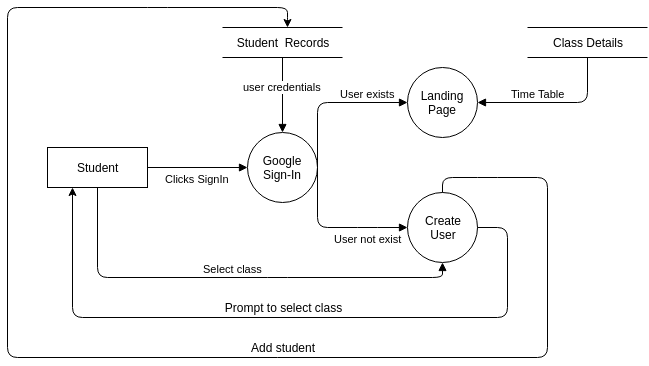
\includegraphics[width=\linewidth]{DFD1.png}
  \caption{DFD project}
\end{figure}

\begin{figure}
  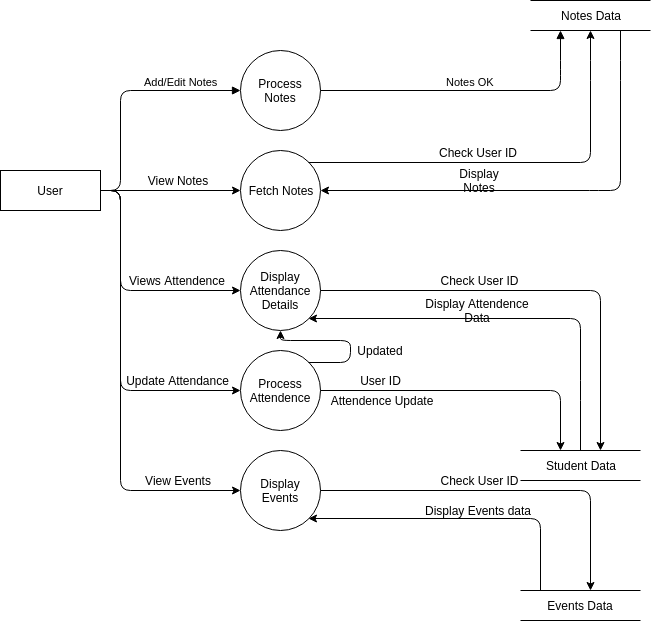
\includegraphics[width=\linewidth]{DFD2.png}
  \caption{DFD}
\end{figure}

%\subsection{Database Design}
%\vspace{1em}
\subsection{Modular Design}

\subsubsection{Login}
This module handles the user authentication and login.
The component is dependent on Google login for its authentication, as we leverage Google signin module to make the tradition of the user into our app much more easier and faster.

Initially when the user logs into the application is when we create an account for them and register them. When the user logs into the application, we get the user to login to their Google account and we can use the Google API top get the user details like user-id, name, email, profile-image etc. This makes it easer for the user as do not have to manually add in their name or profile image. Only thing they will have to manually set is which class they are studying in.

Now from the next time the user logs in, we will directly log them into their account ready to go.

\subsubsection{Landing Page}
The landing page is the most important and most viewed part of the whole application. It encompasses details a user would probably need at that time like upcoming events, which data about the class that is currently going on. It also lets them take down notes which they can later view using the notes module.

For each subject of the day we provide the name of the teacher, time of the class, etc which helps the student to plan for their class.
The place provided to jot down notes for the subject also helps them to take down notes during the classes which will be really useful for them for later reference.

\subsubsection{Notes}
Notes module is aimed at providing an interface for the student( user ) to view all the notes they have taken in the class and go through them.
It is a very useful and powerful utility at the end of a semester as it will let them view all the notes they have in one place and go through them quickly and efficiently.

You can also use the notes view to filter your notes based on the date or the subject which is a really simple but powerful way to summarize a whole semester.

\subsubsection{Attendance}
One another very important module is the Attendance module which lets the student track their attendance for each subject they have. The student on attending or net attending a specific subject class can update their attendance using the attendance module. All the user data is saved in real-time with the backed and they will be able to check their any time.

The per subject nature of the attendance module also helps them to know which subjects they have missed the most and concentrate on them individually.

\subsubsection{Calendar}
The Calendar module is used to view the overview of all the events. It shows you all the events and submissions you have for the future. While the upcoming events module only shows you the close and upcoming events, in the calendar module we can see all the upcoming events in the future.

It has a normal calender like intercase with events listed under the specific dates which makes it much more intuitive and easy.

\vspace{1em}
%\subsection{Input/Output Design}
%\vspace{1em}


\newpage

\section{System Implementation}
\vspace{1em}

\subsection{Sample code}
\vspace{1em}

\lstset{frame=tb,
  language=Python,
  aboveskip=3mm,
  belowskip=3mm,
  showstringspaces=false,
  columns=flexible,
  basicstyle={\small\ttfamily},
  numbers=none,
  numberstyle=\tiny\color{gray},
  keywordstyle=\color{blue},
  commentstyle=\color{dkgreen},
  stringstyle=\color{mauve},
  breaklines=true,
  breakatwhitespace=true,
  tabsize=4
}

\subsubsection{Sample view handlers}
A view handler is a methood which is a specification in django which handles a http request and makes the response.
\vspace{1em}

\begin{lstlisting}
def signin(request):
    if request.method == "POST":
        data = json.loads(request.POST.get('data'))
        sid = data['id']
        if Student.objects.filter(SID=sid).exists():
            return HttpResponse(json.dumps({'exists': True}))
        else:
            classes = [name.class_name for name in Class.objects.all()]
            data = json.dumps({'exists': False, 'options': classes})
            return HttpResponse(json.dumps(data), content_type="application/json")

def get_attendence(request, user_id):
    user = Student.objects.get(SID=user_id)
    attendence_data = user.get_attendence_data()

    print attendence_data
    if len(attendence_data) is 0:
        # quick patch ( issue only if new user already created)
        daytable = user.current_class.get_tt()
        subs = {}
        for key in daytable:
            daysubs = daytable[key].split(',')
            for item in daysubs:
                # if item not in subs:  ( its a dict, lol )
                subs[item] = {'total':0, 'attended':0 }
        attendence_data = subs

    return_data = {}
    return_data['data'] = attendence_data
    return HttpResponse(json.dumps(return_data), content_type="application/json")

def update_attendence(request):
    if request.method == "POST":
        data =  json.loads(request.POST.get('data'))
        user_id = data['id']
        attendence = json.dumps(data['attendance'])

        user = Student.objects.get(SID=user_id)
        user.attendence = attendence
        user.save()
    return_data = { 'status':'OK' }
    return HttpResponse(json.dumps(return_data), content_type="application/json")

\end{lstlisting}

\subsubsection{Url defenitions}
These define the endpoints fot the backend api
\vspace{1em}
\begin{lstlisting}
from django.conf.urls import url
from . import views

urlpatterns = [
    url(r'^$', views.index, name="index"),      # initial request for page
    url(r'^signin/$', views.signin, name='signin'),
    url(r'^create_user/(?P<user_id>[0-9]+)/(?P<user_class>([a-z])+)$', views.create_new_user, name='new_user'),
    url(r'^timetable/(?P<user_id>[0-9]+)$', views.get_timetable, name='timetable'),
    url(r'^notes/(?P<user_id>[0-9]+)$', views.get_notes, name='notes'),
    url(r'^subject_data/(?P<user_id>[0-9]+)$', views.get_sub_data, name='subject_data'),
    url(r'^events/(?P<user_id>[0-9]+)$', views.get_events_dummy, name='events'),
    url(r'^track_data/$', views.get_track_data, name='events'),
    url(r'^calendar/(?P<user_id>[0-9]+)$', views.get_cal_data_dummy, name='events'),
    url(r'^subject_attendence/(?P<user_id>[0-9]+)$', views.get_attendence, name='get_attendence'),
    url(r'^create_user/$', views.create_new_user, name='new_user'),
    url(r'^update_attendence/$', views.update_attendence, name='update_attendence'),
    url(r'^set_track_data/$', views.set_track_data, name='set_track_data'),
]
\end{lstlisting}


\subsubsection{Model defenitions}
These contains the database models for the project
\vspace{1em}

\begin{lstlisting}
 class Subject(models.Model):
    subject_code = models.CharField(verbose_name="Subject Code", max_length=6, primary_key=True)
    subject_title = models.CharField(max_length=60, verbose_name="Subject Title")
    subject_short_name = models.CharField(max_length=3, verbose_name="Abbriviation")
    subject_dep = models.ForeignKey('Department', on_delete=models.CASCADE, verbose_name="Branch")
    subject_sem = models.SmallIntegerField(choices=sem_choices, null=True)

    def __str__(self):
        return self.subject_title


class Teacher(models.Model):
    teacher_name = models.CharField(max_length=40)
    dept = models.ForeignKey('Department', on_delete=models.CASCADE)
    subjects = models.ManyToManyField('Subject', verbose_name="Subjects")

    def __str__(self):
        return self.teacher_name


class Class(models.Model):
    current_sem = models.PositiveSmallIntegerField(choices=sem_choices)
    branch = models.ForeignKey('Department', on_delete=models.CASCADE)
    batch = models.CharField(max_length=1)
    class_name = models.CharField(max_length=10, blank=True)
    timeTable = models.TextField()
    subjects = models.ManyToManyField('Subject', verbose_name='Subjects', through='TaughtBy')

    def save(self, *args, **kwargs):
        self.class_name = str(self.branch) + " " + str(self.current_sem) + str(self.batch)
        super(Class, self).save(*args, **kwargs)

    def get_subs(self):
        subs = [subject.subject_short_name for subject in self.subjects.all()]
        return subs

    def get_tt(self):
        tt_string = str(self.timeTable)
        tt_string = tt_string.splitlines()
        days = ['monday', 'tuesday', 'wednesday',
                'thursday', 'friday']
        tt_dict = {}
        for i in range(5):
            tt_dict[days[i]] = tt_string[i]

        return tt_dict

    def __str__(self):
        return str(self.class_name)

    class Meta:
        verbose_name_plural = "Classes"
\end{lstlisting}

\lstset{frame=tb,
  language=HTML,
  aboveskip=3mm,
  belowskip=3mm,
  showstringspaces=false,
  columns=flexible,
  basicstyle={\small\ttfamily},
  numbers=none,
  numberstyle=\tiny\color{gray},
  keywordstyle=\color{blue},
  commentstyle=\color{dkgreen},
  stringstyle=\color{mauve},
  breaklines=true,
  breakatwhitespace=true,
  tabsize=4
}

\subsubsection{Base html template}
A basic html template for a page
\vspace{1em}
\begin{lstlisting}
<div class='fullpage'>
    <div class='leftpane pane'>
        <div class='card small heading' id='lheading'>
            Navigation
        </div>
        <div class='navel' id='home'>
            <i class="fa fa-home" aria-hidden="true"></i><br>
            Home
        </div>
        <div class='navel' id='notes'>
            <i class="fa fa-sticky-note" aria-hidden="true"></i><br>
            Notes
        </div>
        <div class='navel' id='attendece'>
            <i class="fa fa-child" aria-hidden="true"></i><br>
            Attendence
        </div>
        <div class='navel' id='calender'>
            <i class="fa fa-calendar" aria-hidden="true"></i><br>
            Calender
        </div>
        <div class='navel' id='about'>
            <i class="fa fa-info-circle" aria-hidden="true"></i><br>
            About
        </div>
    </div>
    <div class='midpane pane'>
        <div id='mheading'>
            <i class="fa fa-bars" aria-hidden="true" id="hamburger-menu-button"></i>
            <img id="profile-image" src="" alt="profile">
            <div id='profile-name'></div>
            <i class="fa fa-asterisk" aria-hidden="true" id="upcoming-menu-button"></i>
        </div>
        <div id='mcontent'>
        </div>
    </div>
    <div class='rightpane pane'>
        <div class='card small heading' id='rheading'>
            Upcoming
        </div>
        <div class='content' id='rcontent'>
        </div>
    </div>
</div>
\end{lstlisting}


\lstdefinelanguage{JavaScript}{
  keywords={typeof, new, true, false, catch, function, return, null, catch, switch, var, if, in, while, do, else, case, break},
  keywordstyle=\color{blue}\bfseries,
  ndkeywords={class, export, boolean, throw, implements, import, this},
  ndkeywordstyle=\color{blue}\bfseries,
  identifierstyle=\color{black},
  sensitive=false,
  comment=[l]{//},
  morecomment=[s]{/*}{*/},
  commentstyle=\color{purple}\ttfamily,
  stringstyle=\color{red}\ttfamily,
  morestring=[b]',
  morestring=[b]"
}

\lstset{frame=tb,
  language=Javascript,
  aboveskip=3mm,
  belowskip=3mm,
  showstringspaces=false,
  columns=flexible,
  basicstyle={\small\ttfamily},
  numbers=none,
  numberstyle=\tiny\color{gray},
  keywordstyle=\color{blue},
  commentstyle=\color{dkgreen},
  stringstyle=\color{mauve},
  breaklines=true,
  breakatwhitespace=true,
  tabsize=4
}

\subsubsection{Sample module in js}
Our js file in a modular design and the below show is the code to initialize a user account.
\vspace{1em}

\begin{lstlisting}
InitializeUser = function(user){
    this.class_name = 'initialize_user';
    this.user = user;
}
InitializeUser.prototype.get_data_from_server = function(callback){
    var self = this;
    if (callback === undefined) { callback=function(){} }
    $.get(server_address+'/events/'+fuid, function(upcoming_events){
        self.events = upcoming_events['data'];
        callback()
    })
}
InitializeUser.prototype.init = function(events){
    var self = this
    this.get_data_from_server(function(){
        self.populate_user_profile();
        self.populate_upcoming();
        self.click_handlers();
    })
}
InitializeUser.prototype.populate_user_profile = function(){
    $('#profile-name').html(this.user['name']);
    $('#profile-image').attr('src', this.user['photo']);
    $('#popup-profile-name').html(this.user['name']);
    $('#popup-profile-image').attr('src', this.user['photo']);
    $('#popup-profile-email').html(this.user['email']);
}
InitializeUser.prototype.populate_upcoming = function(){
    var self = this;
    htmlstr = '';
    for( var i=0, len=this.events.length; i<len; i++ ){
        htmlstr +=
            "<div class='card small event' data-event="+i+">"+
                "<div class='card tiny date-card'>"+
                    this.events[i]['due']+
                "</div>"+
                "<div class='card tiny subject-card'>"+
                    "<span class='span violet name'>title</span><span class='span white span-content'>"+ this.events[i]['name']+ "</span>"+
                "</div>"+
                "<div class='card tiny subject-card'>"+
                    "<span class='span green name'>subject</span><span class='span white span-content'>"+ this.events[i]['subject']+ "</span>"+
                "</div>"+
                "<div class='card tiny subject-card'>"+
                    "<span class='span blue name'>submission</span><span class='span white span-content'>"+ this.events[i]['to']+ "</span>"+
                "</div>"+
            "</div>"
    }
    $('#rcontent').html(htmlstr);

    // Now set up the click handlers
    event_cards = $('.event');
    for(var i = 0, len = event_cards.length; i<len; i++){
        $(event_cards[i]).click(function(){
            event_data = self.events[$($(this)[0]).data('event')]
            el_main = $('#event-popup').children()
            el_date = $($(el_main[1]).children()[1]).text(event_data['due'])
            el_title = $($(el_main[2]).children()[1]).text(event_data['name'])
            el_subject = $($(el_main[3]).children()[1]).text(event_data['subject'])
            el_submission = $($(el_main[4]).children()[1]).text(event_data['to'])
            el_desc = $($(el_main[5]).children()[3]).text(event_data['description'])
            // console.log(el_date, el_subject, el_submission, el_desc)
            $($('#event-popup').parent()).css('display', 'flex');
        });
    }
    $($('#event-popup').parent()).click(function(){
        $($('#event-popup').parent()).css('display', 'none');
    });
}
InitializeUser.prototype.click_handlers = function(){
    // User logout
    $('#popup-profile-signout-button').click(function(){
        var auth2 = gapi.auth2.getAuthInstance();
        auth2.signOut().then(function () {
            console.log('User signed out.');
        });
        $('#login-popup').css('display', 'flex');
        $($('#signout-popup').parent()).css('display', 'none');
    });
    // Handle sinout popup remove click
    $($('#signout-popup').parent()).click(function(){
        $($('#signout-popup').parent()).css('display', 'none');
    });
    $('#signout-popup').click(function(e){
        e.stopPropagation();
    });
    // Open up the signout popup
    $('#profile-image').click(function(){
        $($('#signout-popup').parent()).css('display', 'flex');
    });


    //other handles (menu items)
    $('#home').click(function(){
        new Home().init()
    });
    $('#notes').click(function(){
        new NotesView().init()
    });
    $('#about').click(function(){
        new AboutView().init()
    });
    $('#attendece').click(function(){
        new AttendenceView().init()
    });
    $('#calender').click(function(){
        new CalenderView().init()
    });
}
\end{lstlisting}

\subsubsection{Sample CSS file}
In here we define the styling for the elements
\vspace{1em}

\begin{lstlisting}
.fullpage{
    width: 100%;
    height: 100%;
    overflow: hidden;
}
.pane{
    padding: 10px;
    margin: 10px;
    margin-top: 30px;
    margin-bottom: 30px;
    float:left;
    border-radius: 1px;
    box-shadow: 0px 0px 2px 0px rgba(0,0,0,0.75);
    background-color: #fff;
}
.leftpane{
    width: 20vw;
    height: calc(100% - 80px);
    transition-property: width, visibility;
    transition-duration: 0.5s;
    z-index: 100;
    overflow: auto;
}
.midpane{
    width: calc(60vw - 120px);
    height: calc(100% - 80px);
    transition-property: width;
    transition-duration: 0.5s;
    overflow: hidden;
}
.rightpane{
    width: 20vw;
    height: calc(100% - 80px);
    transition-property: width;
    transition-duration: 0.5s;
    z-index: 100;
    overflow: auto;
}
@media screen and (max-width: 1050px){
    /* Remove navigation */
    .leftpane{
        display: none;
    }
    .rightpane{
        width: 230px;
    }
    .midpane{
        /* width: calc(100vw - 40px); */
        width: calc(100vw - 320px);
    }
}
\end{lstlisting}


\newpage

\subsection{Screenshots}
\vspace{1em}

\begin{figure}
  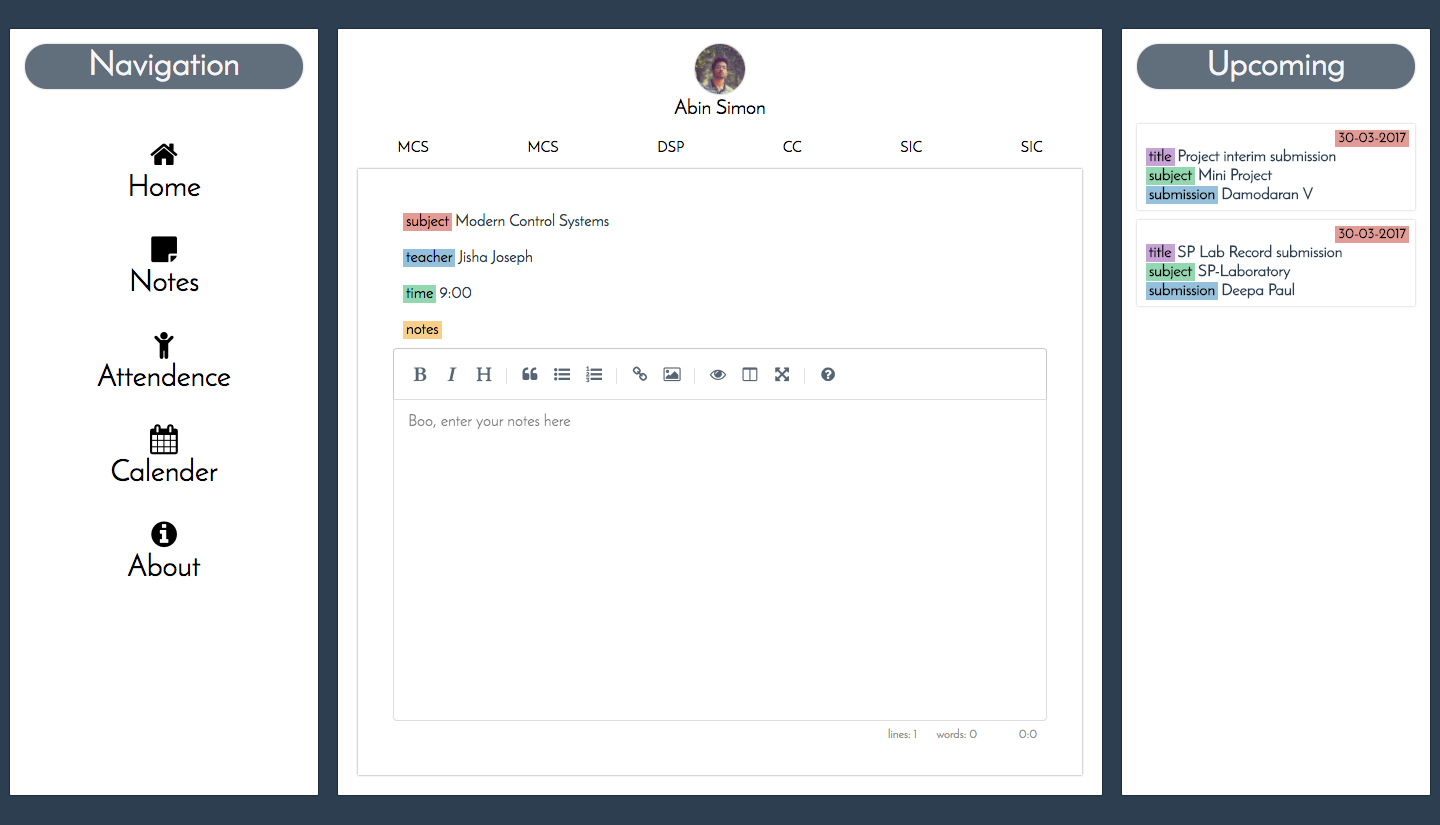
\includegraphics[width=\linewidth]{landingpage.png}
  \caption{Landing page}
\end{figure}

\begin{figure}
  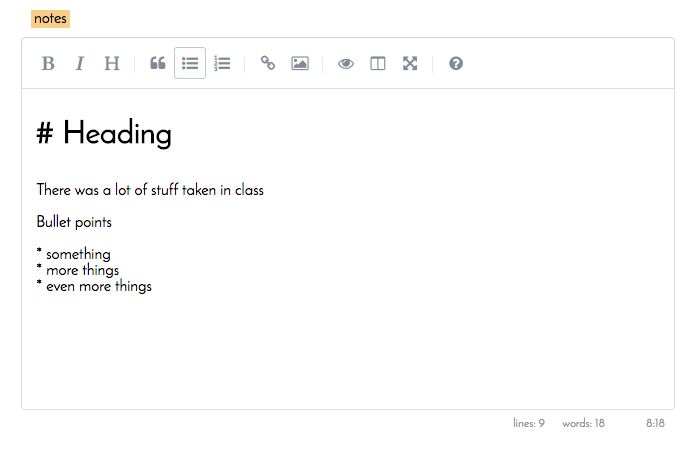
\includegraphics[width=\linewidth]{notesmd.png}
  \caption{Write notes in markdown}
\end{figure}

\begin{figure}
  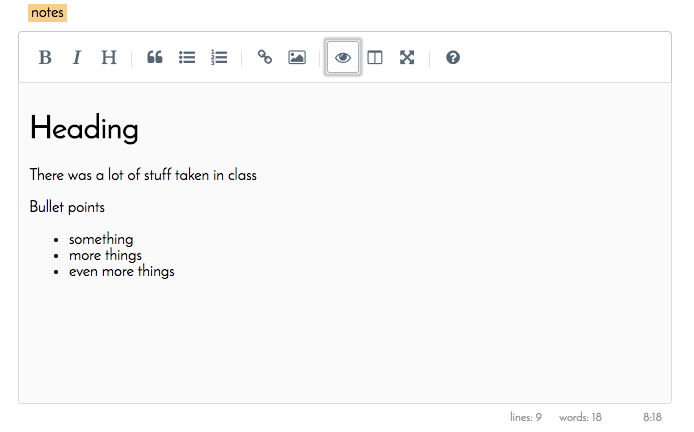
\includegraphics[width=\linewidth]{notescompiled.png}
  \caption{Compiled the written notes to actual contet in place}
\end{figure}

\begin{figure}
  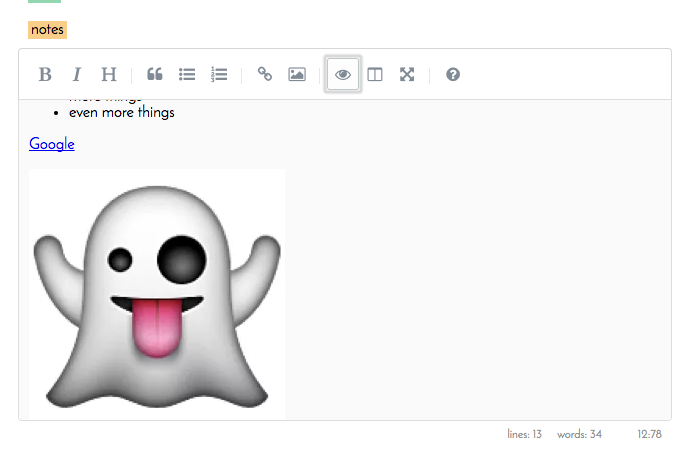
\includegraphics[width=\linewidth]{noteswithimages.png}
  \caption{You can even have notes with images and links}
\end{figure}

\begin{figure}
  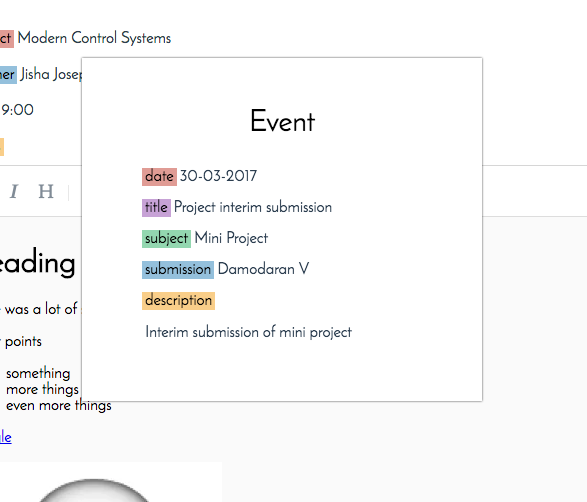
\includegraphics[width=\linewidth]{eventinfo.png}
  \caption{Detailed information about upcoming events}
\end{figure}

\begin{figure}
  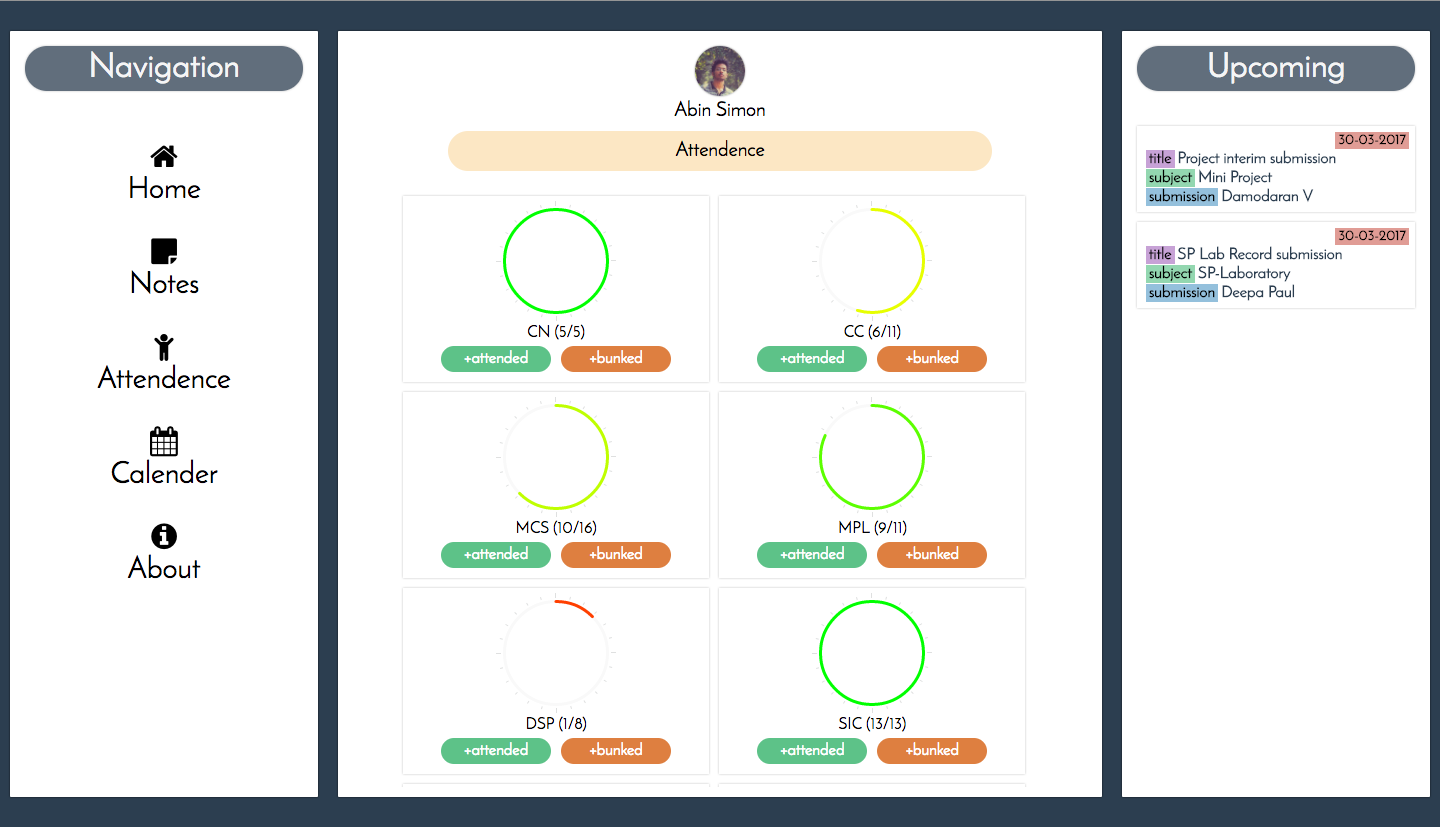
\includegraphics[width=\linewidth]{attendance.png}
  \caption{View and update attendace}
\end{figure}

\begin{figure}
  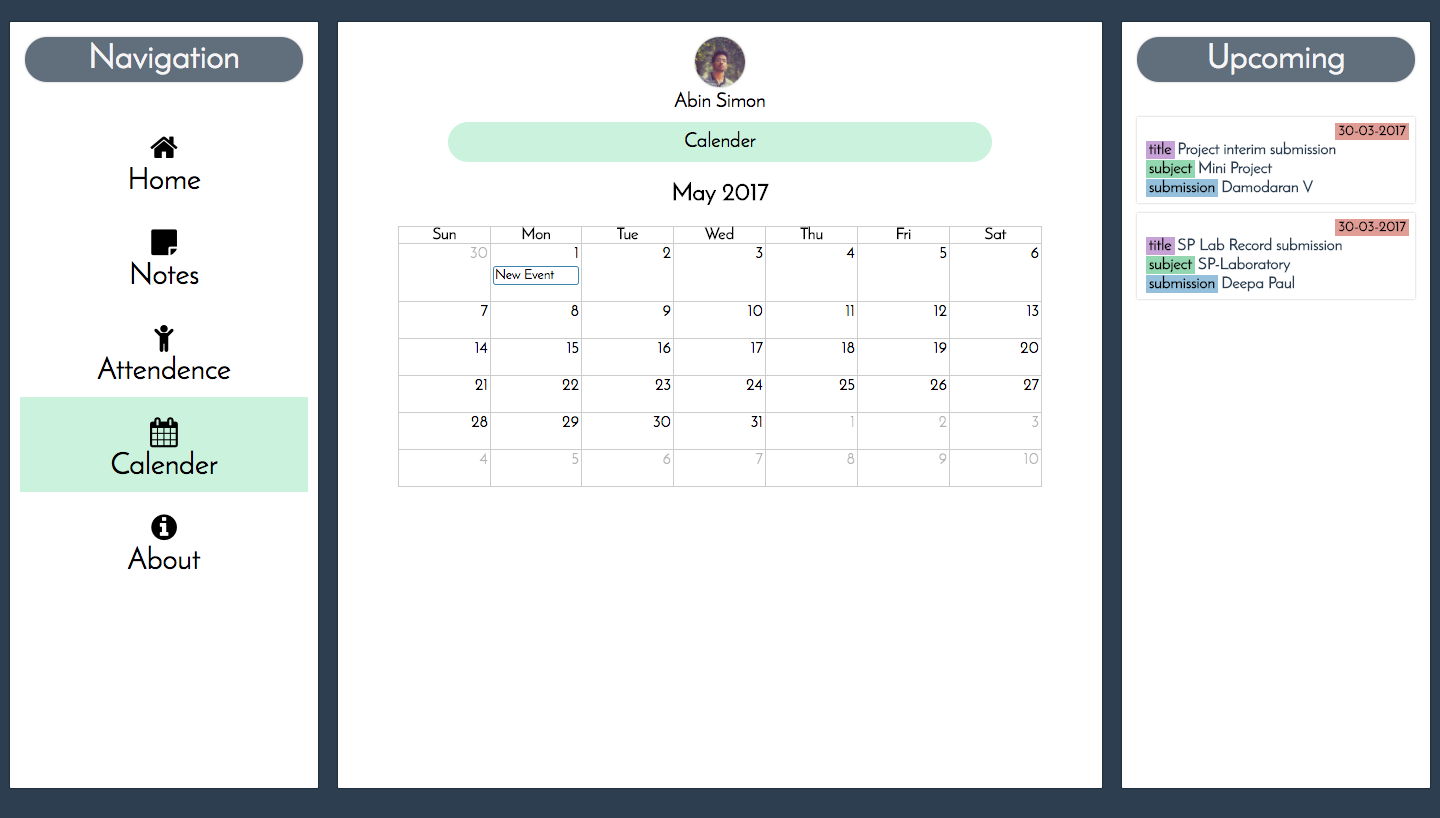
\includegraphics[width=\linewidth]{calendar.png}
  \caption{Calendar entries for events}
\end{figure}

\begin{figure}
  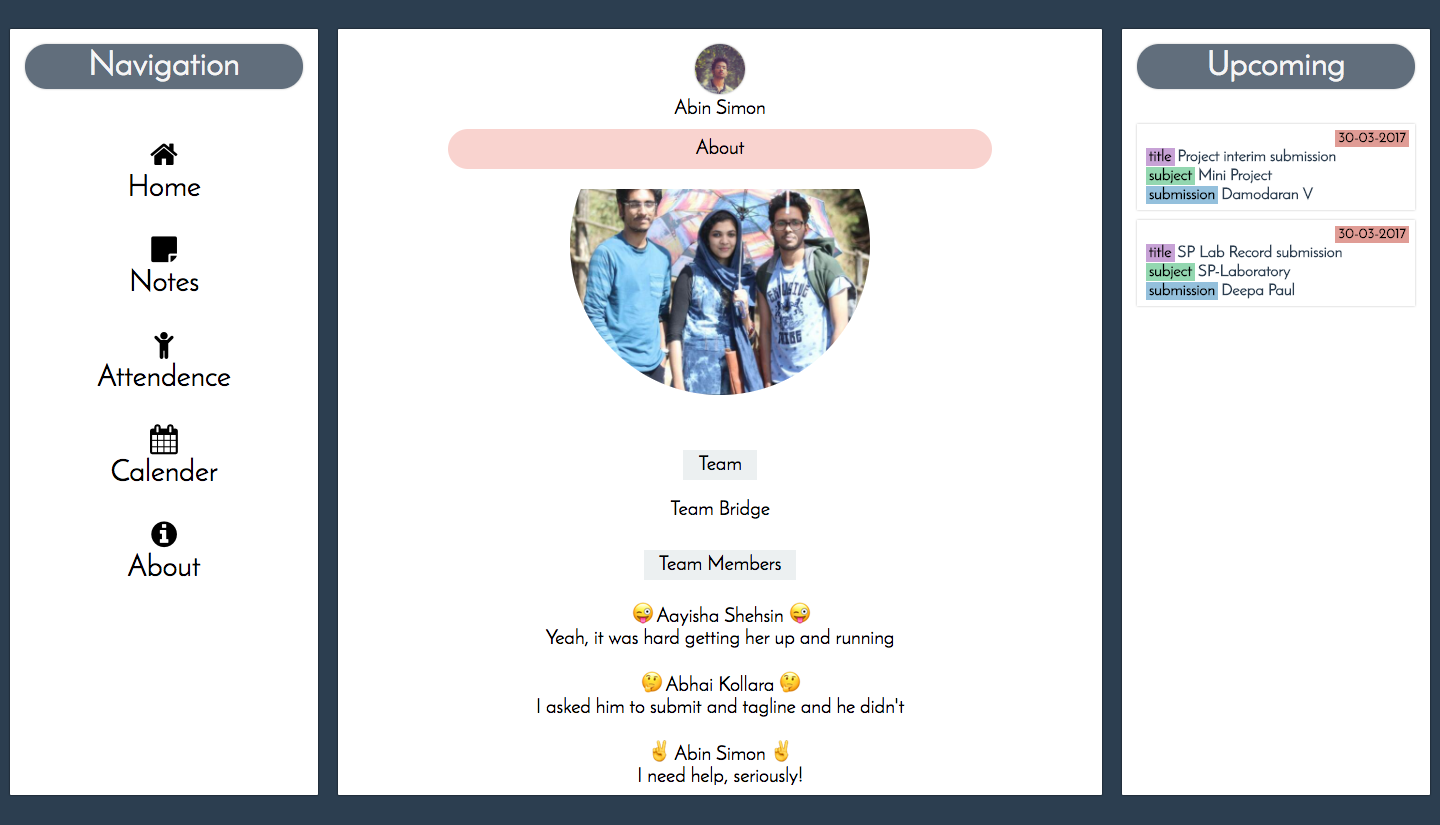
\includegraphics[width=\linewidth]{aboutpage.png}
  \caption{About page}
\end{figure}

\begin{figure}
  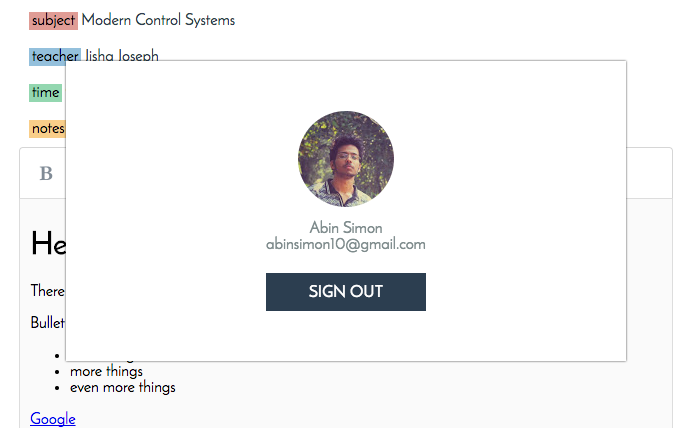
\includegraphics[width=\linewidth]{signoutpopup.png}
  \caption{Popup to sign out of the system}
\end{figure}

\begin{figure}
  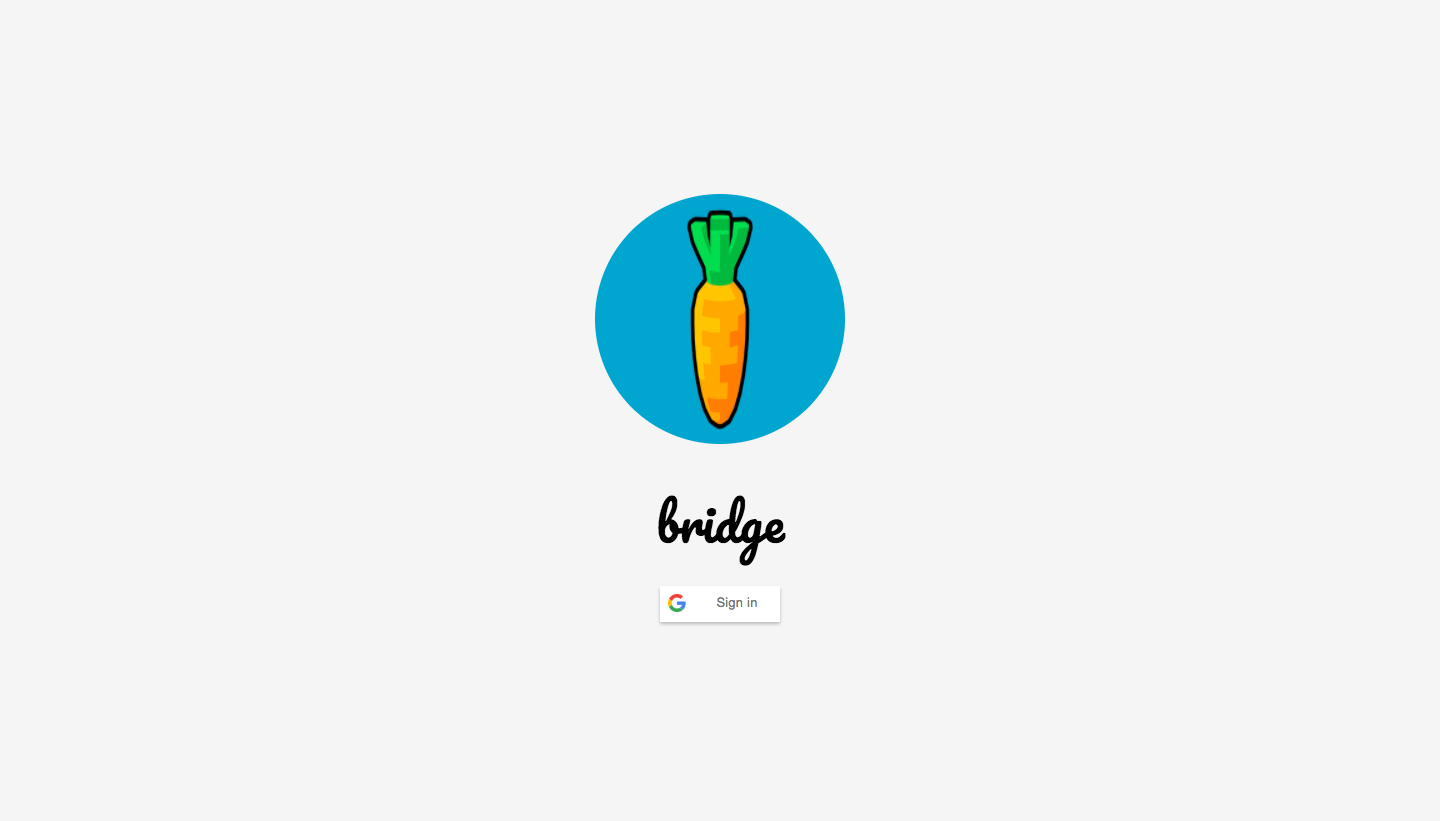
\includegraphics[width=\linewidth]{loginpopup.png}
  \caption{Interface for loggin into the app}
\end{figure}

\begin{figure}
  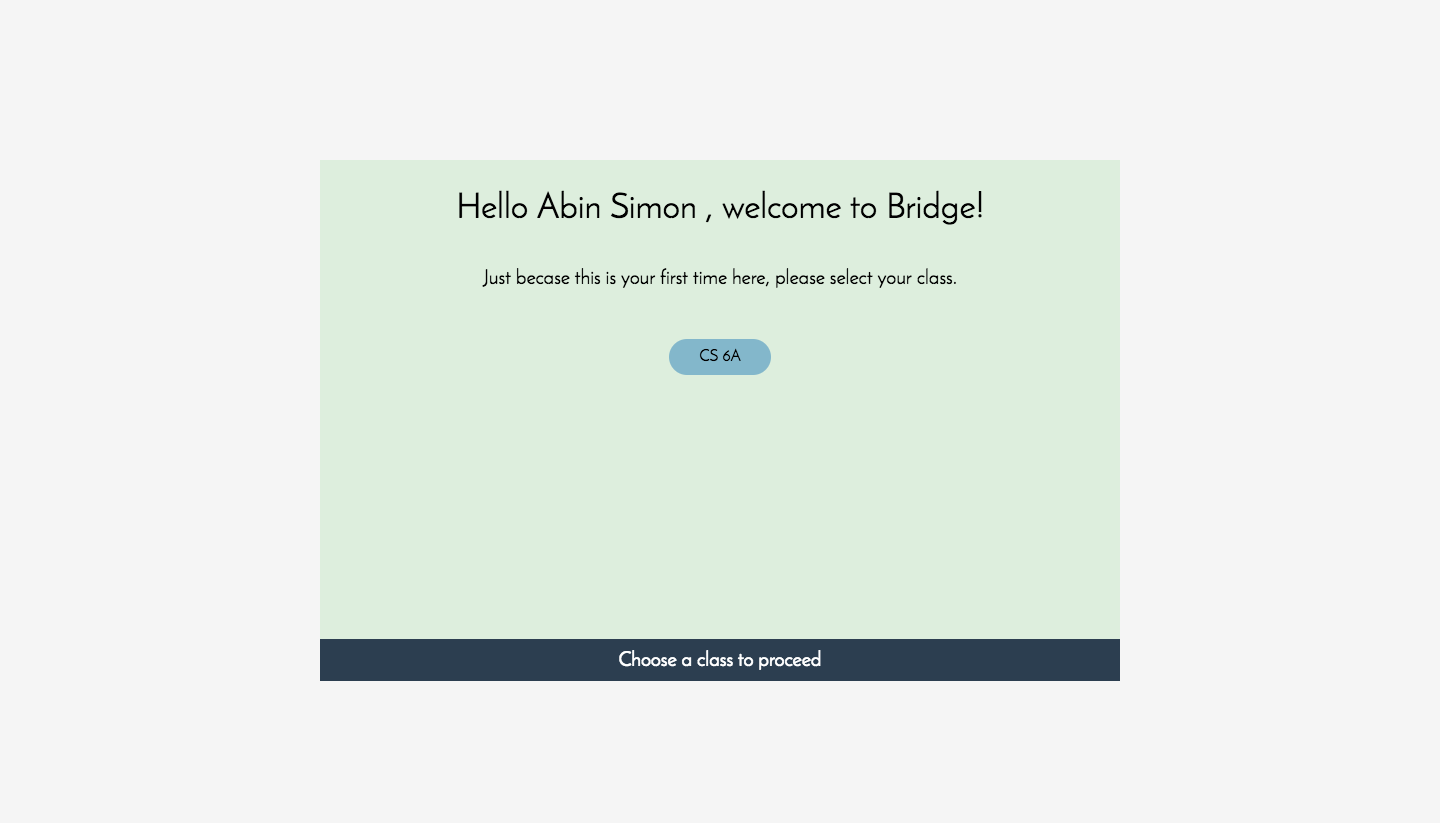
\includegraphics[width=\linewidth]{newuserpopup.png}
  \caption{Interface if the user is a new one so that he can choose a class}
\end{figure}

\begin{figure}
  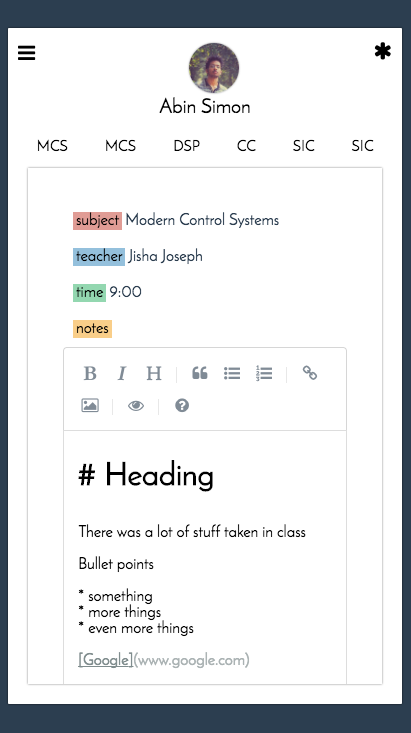
\includegraphics[width=\linewidth]{mobilelanding.png}
  \caption{Landing page on mobile}
\end{figure}


\begin{figure}
  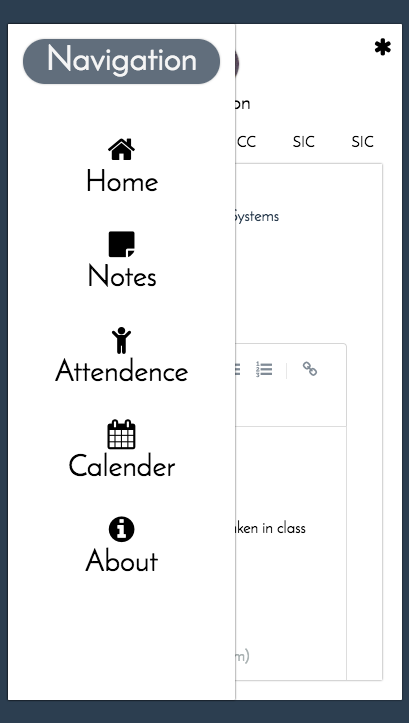
\includegraphics[width=\linewidth]{mobilenav.png}
  \caption{Navigation pane on mobile}
\end{figure}

\begin{figure}
  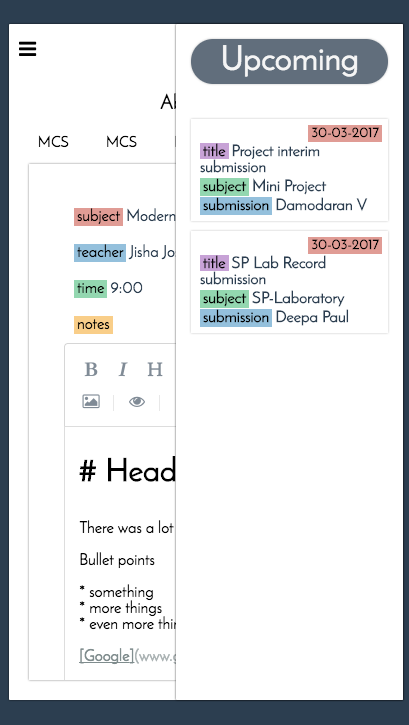
\includegraphics[width=\linewidth]{mobileupcoming.png}
  \caption{Upcoming event display on mobile}
\end{figure}

\begin{figure}
  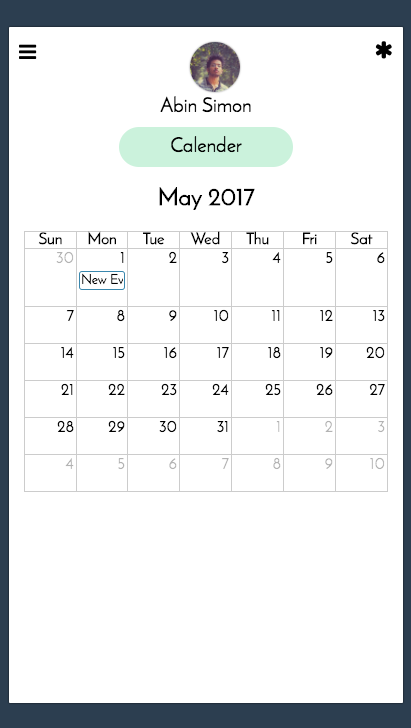
\includegraphics[width=\linewidth]{mobilecalendar.png}
  \caption{Calendar display on mobile}
\end{figure}


\newpage


\section{System Testing}
\vspace{1em}

The aim of the system testing process was to determine all defects in our project. The program was subjected to a set of test inputs and various observations were made and based on these observations it will be decided whether the program behaves as expected or not.

Our Project went through four levels of testing
\begin{itemize}
\item Unit testing
\item Integration testing
\item System testing
\item Component Interface Testing
\end{itemize}

\subsection{Unit testing}
Unit testing is undertaken when a module has been created and successfully reviewed. In order to test a single module we need to provide a complete en- vironment i.e. besides the module we would require. The procedures which belong to other modules that the module under test calls non local data structures that module access a procedure to call the functions of the mod- ule under test with appropriate parameters. Unit testing was done on each and every module that is described under module wise description.

\subsection{Integration testing}
In this type of testing we test various integration of the project module by providing the input. The primary objective is to test the module interfaces in order to ensure that no errors are occurring when one module invokes the other module.

\subsection{System testing}
System testing, or end-to-end testing, tests a completely integrated system to verify that it meets its requirements. For example, a system test might involve testing a logon interface, then creating and editing an entry, plus sending or printing results, followed by summary processing or deletion (or archiving) of entries, then logoff.
In addition, the software testing should ensure that the program, as well as working as expected, does not also destroy or partially corrupt its operating environment or cause other processes within that environment to become inoperative (this includes not corrupting shared memory, not consuming or locking up excessive resources and leaving any parallel processes unharmed by its presence).

\subsection{Component interface testing}
The practice of component interface testing can be used to check the handling of data passed between various units, or subsystem components, beyond full integration testing between those units. The data being passed can be con- sidered as ”message packets” and the range or data types can be checked, for data generated from one unit, and tested for validity before being passed into another unit. One option for interface testing is to keep a separate log file of data items being passed, often with a timestamp logged to allow analysis of thousands of cases of data passed between units for days or weeks. Tests can include checking the handling of some extreme data values while other interface variables are passed as normal values. Unusual data values in an interface can help explain unexpected performance in the next unit. Com- ponent interface testing is a variation of black box testing, with the focus on the data values beyond just the related actions of a subsystem component.

\newpage

%% \section{Future Scope}
%% \vspace{1em}
%% The  system in the future expects to be more inevery way. Automate more components and also create new components for both teachers and students alike.


%% \newpage

\section{Conclusion}
\vspace{1em}
A conscious effort has been made while creating and developing the software package ,making use of existing tools, techniques and resource that would cater the demands .The project has shown us the finer aspect of database management system.
While making the system, an eye has been kept on making it as user-friendly, as cost-effective as possible. As such one may hope that the system will be acceptable to any user and will adequately meet his/her needs. The entire project is menu assisted and highly interactive. On trial run the performance was found to be satisfactory. But as in case of any system development processes , there were are a number of shortcomings, there have been some shortcomings in the development of this system also. Thus project is still under modification.

\newpage


\section{Reference}
\vspace{1em}
\begin{itemize}
\item Learn python the hard way (https://learnpythonthehardway.org/)
\item Django official docs (https://docs.djangoproject.com/en/1.11/)
\item Django Girls Tutorial (https://tutorial.djangogirls.org/en/index.html)
\item W3 Schools (https://www.w3schools.com/)
\item Tutorials point (https://www.tutorialspoint.com/)
\item Stack Overflow (http://stackoverflow.com/)
\item Udacity (https://in.udacity.com/)
\item Coursera (https://www.coursera.org/)
\end{itemize}


\newpage


\end{document}
